\chapter{Stand der Technik -- Einführung in die Beacon-Technologie}
Der erste Teil dieses Kapitels beschäftigt sich mit der Entstehungsgeschichte von iBeacons und nachfolgend mit deren Funktionsweise. Hier wird besonders auf die technischen Möglichkeiten der Technologie eingegangen. Im letzten Abschnitt wird erläutert, wo Beacon-Systeme zum Einsatz kommen und wie aktuelle Lösungsansätze für die Planung der dafür nötigen Infrastruktur aufgebaut sind. Anschließend wird aus den gegebenen Charakteristika der Beacons und der momentanen genutzten Fähigkeiten differenziert und eine Aussicht auf ein zukünftiges Konzept zu einer besseren Nutzung gegeben.
\section{Entwicklungsgeschichte}
Der Grundstein für die Beacon-Technologie legte die Firma Nokia im Jahre 2006. Damals entwickelte die Firma den neuen Standard \textit{Wibree} für die Funkübertragung, der den alten Bluetooth-Standard ersetzen sollte. Mit der Neuentwicklung versprach man sich im Gegensatz zu Bluetooth einen geringeren Stromverbrauch und geringere Produktionskosten, bei gleichbleibenden Übertragungsraten. Ab dem Jahr 2009 wurde der Bluetooth-Standard um Wibree ergänzt und erst unter den Bezeichnungen \textit{Ultra Low Power Bluetooth} (ULP) und dann später als \textit{Bluetooth Low Energy} (BLE) darin aufgenommen \cite{Wib2BLE} und anschließend als \textit{Bluetooth Smart} vermarktet. Da viele Hersteller von mobilen Geräten in ihren Datenblättern die Unterstützung von BLE nicht explizit erwähnen, findet sich meistens folgendes Logo \ref{BLElogo} in den Produktbeschreibungen und lässt erkennen, ob die Geräte den neuen Standard unterstützen. \\ \\
Die Idee der Nutzung von Bluetooth Low Energy zur Indoor-Lokalisierung stammt dabei von der Firma Apple Inc. und wurde von ihr im Jahre 2013 auf der WWDC (Worldwide Developers Conference)\cite{Apple} unter dem Namen \textit{iBeacon} angekündigt. Obwohl zu dem Zeitpunkt noch kein fertiges Gerät zur Verfügung stand, wurde diese Technologie als Neuerung in Apples mobilem Betriebssystem iOS 7 vorgestellt. Jedoch verzichtet Apple seither auf die Produktion von iBeacons, was andere Unternehmen nutzen um selbst in den Markt einzusteigen. Deren Produkte wurden darauf in Beacons umbenannt und unterstützen zusätlich die mobilen Betriebssysteme Android ab Version 4.3, Windows Phone 8 und neue die neueste Version von Blackberries OS \cite{Bibel}. Somit wäre die Beacon-Technologie mit der nötigen Hardware-Unterstützung in mittlerweile über 99,5\% aller mobilen Geräte (Smartphones, Tablets, Smartwatches, etc.) weltweit nutzbar \cite{MobGerSt}. \par\bigskip
\begin{figure}[H]
\centering

\includegraphics[scale=0.07]{Bilder/BLE.png} 
\caption{Offizielles Bluetooth Smart Logo \cite{BLElogo}}
\label{BLElogo}
\end{figure}
%\begin{figure}[H]
%\centering
%
\includegraphics[scale=0.5]{Bilder/iBeaconLogo.png} 
%\caption{Offizielles iBeacon Logo \cite{iLogo}}
%\label{iLogo}
%\end{figure}
%
\newpage
\section{Aufbau und Funktionsweise von Beacons} 
\begin{wrapfigure}{r}{6cm}
\begin{flushright}
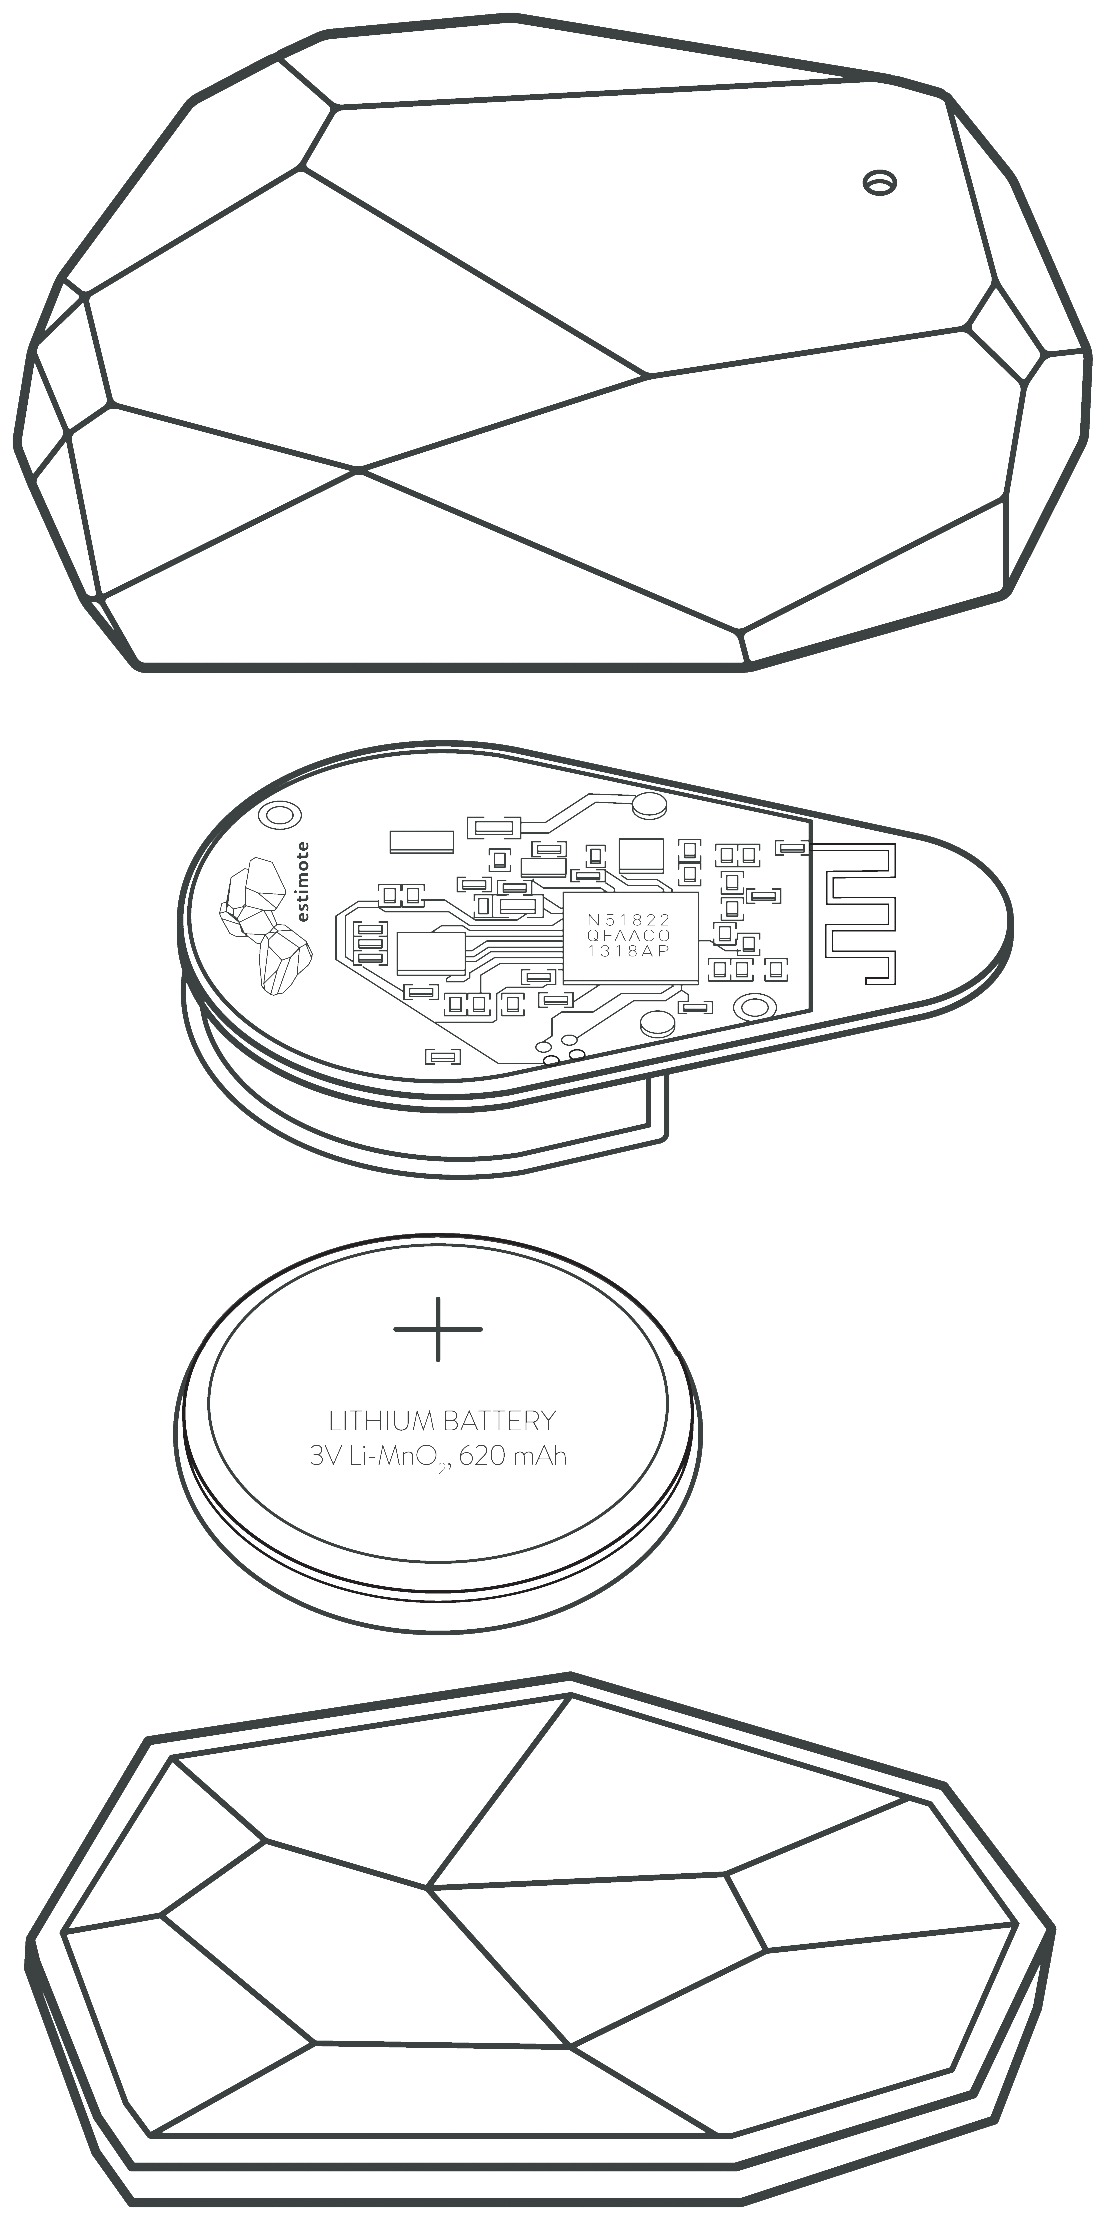
\includegraphics[scale=0.07]{Bilder/BeaconSchicht.png}
\caption{Explosionszeichnung Beacon \cite{BeaEx}}
\label{fig:BeaEx}
\begin{picture}(0,0)
\put(-150,177){Schutzhülle}
\put(-85,182){\line(1,0){25}}
\put(-150,137){Platine}
\put(-110,142){\line(1,0){50}}
\put(-150,100){Batterie}
\put(-100,105){\line(1,0){40}}
\put(-150,60){Silikonplatte}
\put(-80,65){\line(1,0){20}}
\end{picture}
\end{flushright}
\end{wrapfigure}
Die Grundbausteine der kleinen Leuchtfeuer sind in der rechten Abbildung \ref{fig:BeaEx} ersichtlich, in der ein \textit{Estimote Beacon} der Firma Estimote Inc. in seinen einzelnen Bestandteile untergliedert ist. Ein Beacon misst ungefähr 5,5 cm $\times$ 3,5 cm $\times$ 1,5 cm in Länge, Breite und Höhe und ist dabei 50 g schwer. Zur Anbringung der Beacons an Wänden, Decken usw. dient die auf der Rückseite befindliche Silikonplatte. Diese haftet an nahezu jeder glatten Oberfläche und kann mithilfe von Wasser sehr einfach gereinigt werden. Somit können die Beacons im Grunde unzählige Male angebracht und wieder abgenommen werden. Die äußere Schutzhülle besteht dabei ebenfalls aus einem Silikon und schützt die inneren Bauteile. Zu den inneren Komponenten gehören die Platine mit dem darauf verlöteten Nordic nRF51822 Chip (32-Bit ARM Cortex M0 CPU mit 256 kB Flash-Speicher und dem 2,4 GHz BLE-Sendemodul) \cite{nRF5}, einer Antenne und eine Knopfbatterie zur autarken Stromversorgung. Die Beacons haben eine variable Sendeleistung von 4dBm bis -30dBm (entspricht einer Leistung von 2,512 Milliwatt bis 1 Microwatt) und übertragen ihre Daten in Intervallen von 50 bis 0,5 Hertz. Die Kommunikation verläuft dabei bidirektional, d.h. vom Beacon zum Empfangsgerät und zurück. Während die Kommunikation von Beacon zu einem mobilen Gerät dazu dient, die Lokalisierung des Gerätes zu ermöglichen, dient die Kommunikation vom Smartphone, Tablet, etc. zum Beacon zu dessen Programmierung und zur Überprüfung des Betriebszustandes, wie z.B. dem Akku-Zustand. \\ \\
Die bei der Signalübertragung verwendete Protokoll-Architektur Bluetooth Low Energy sendet dabei im 2,4 Ghz Band, welches ebenfalls von den Protokollen 802.11 ac/a/b/g/n, älteren Bluetooth-Standards, ZigBee, NFC, etc. genutzt wird. Eine kompakte Übersicht zu den einzelnen Varianten und deren Eigenschaften findet sich im Anhang in Bild \ref{fig:FUE}. Die Vorteile vom 2,4 Ghz Band gegenüber anderen Frequenzbändern ergeben sich aus einer großen Reichweite der Funksignale und einer geringen Größe der Antenne für deren Erzeugung. Jedoch besitzt dieses Band auch gewisse Nachteile, die bei der Auslegung von Beacon-Konfiguartionen beachtet werden müssen. Die Verwendung des Protokolls im 2,4 Ghz Band ist dabei historisch bedingt und nahezu alternativlos, da sie zu den ISM-Bändern \cite{BuNet} zählt und nur diese somit frei nutzbar sind. Durch die Benutzung des 2,4 Ghz Bandes für die Datenübertragungen in WLAN oder Bluetooth treten bei vermehrter Nutzung des Bandes leicht Störungen in den Übertragungen auf. Somit hängt die Qualität der Signale und schlussendlich auch die Lokalisierungsgenauigkeit von der lokalen Auslastung des 2,4 Ghz Bandes ab. Desweiteren können auch zwischen Sender und Empfänger befindlichen physischen Objekte einen störenenden Faktor auf die Empfangsqualität ausüben. In den Bildern \ref{fig:Wand} und \ref{fig:Hand} ist eine mögliche Beeinträchtigung der Empfangsqualität von BLE-Signalen durch eine im Sichtfeld befindliche Wand oder eines menschlichen Körpers dargestellt. Denn durch die physikalischen Eigenschaften des 2,4 Ghz Bandes werden die Funksignale durch Materialien wie Wasser und Stahl besonders gut absorbiert. Da die meisten Gebäude aus Stahlbeton errichtet wurden und der menschliche Körper aus einem großen Anteil aus Wasser besteht, wirken sich diese Umstände besonders negativ auf die Qualität der Signale und am Ende auf die Anwendung der BLE-Technik für die Lokalisierung von Menschen in Gebäuden aus. Jedoch sei dies nur am Rande erwähnt und würde unter zusätzlicher Betrachtung dieser Aspekte den zeitlichen Rahmen dieser Arbeit in großem Ausmaß sprengen. Zusammenfassend werden hier noch einmal die Gründe für eine Qualitätsminderung der Lokalisierung festgehalten: die Schwächung der Signale an Objekten, die Phasenauslöschung durch andere Signalquellen und unberechenbaren Reflexionen.\\ \\
\begin{figure}[H]
$\begin{minipage}[b]{7cm}
\centering
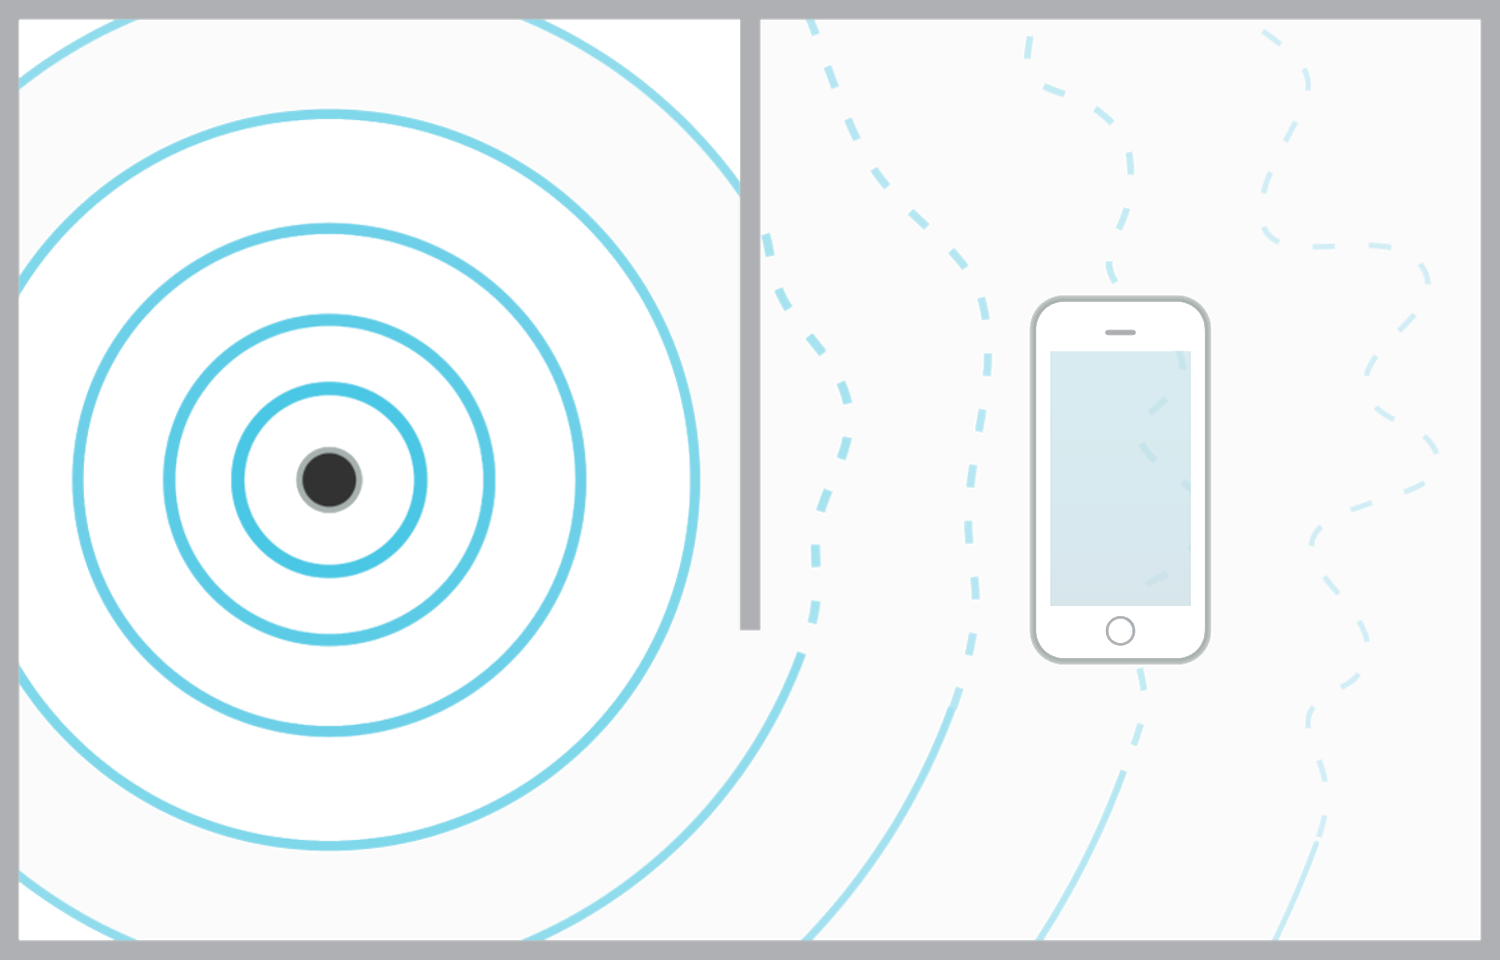
\includegraphics[scale=0.13]{Bilder/Wand.png} 
\caption{Signalschwächung durch Objekte, z.B. Wände \cite{GSwiB}}
\label{fig:Wand}
\end{minipage}
\hspace{3cm}
\begin{minipage}[b]{7cm}
\centering
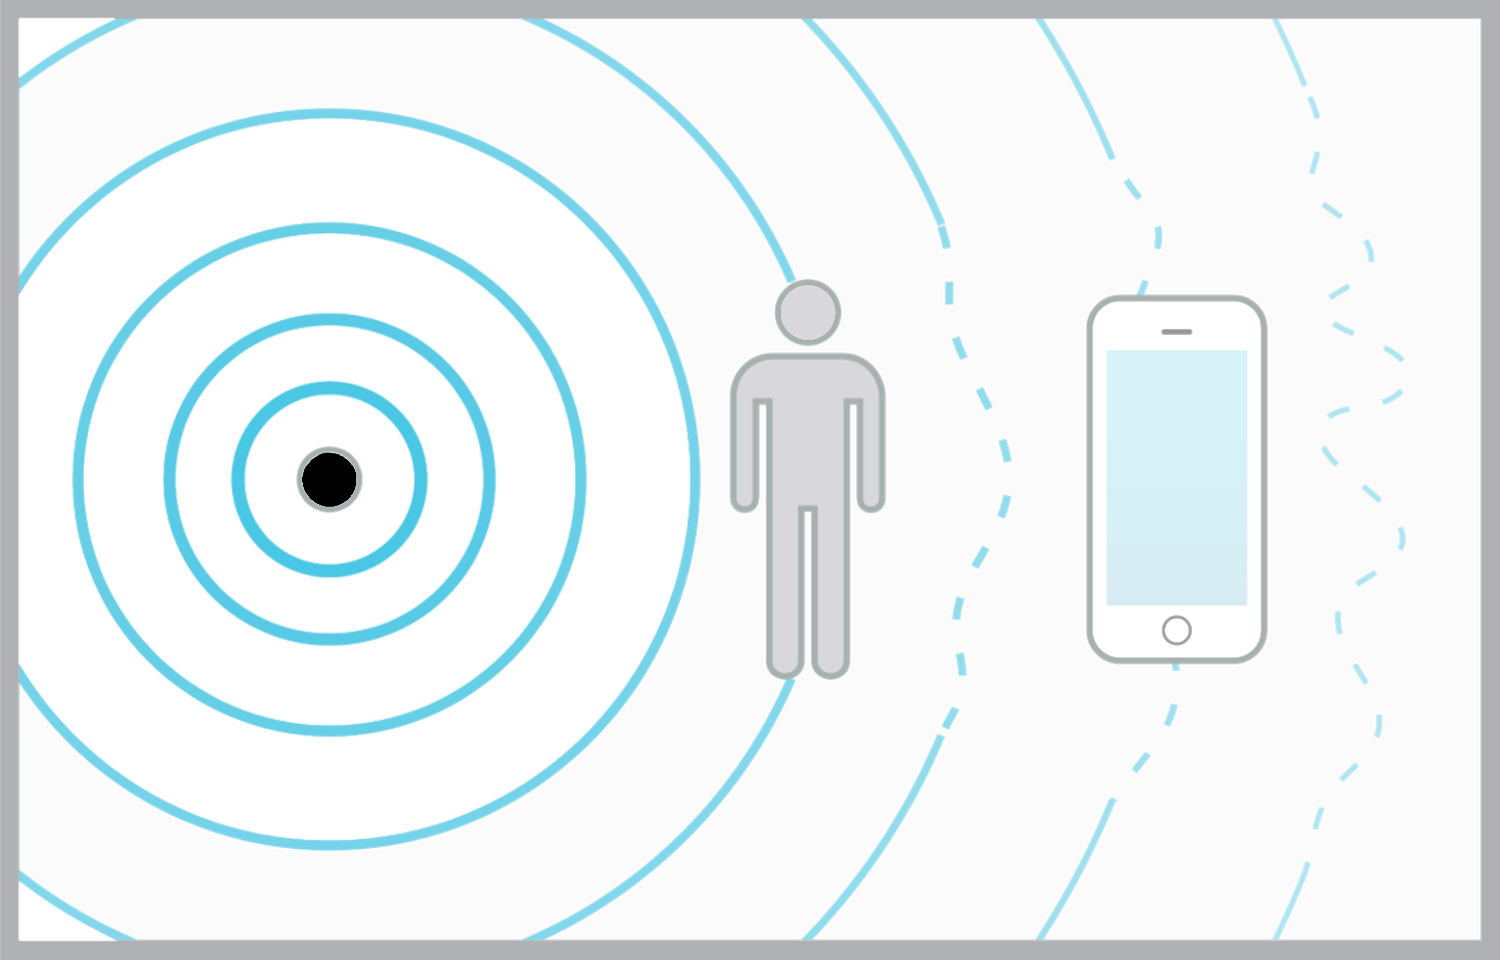
\includegraphics[scale=0.13]{Bilder/Hand.png} 
\caption{menschliche Körper blockieren zusätzlich die Signale \cite{GSwiB}}
\label{fig:Hand}
\end{minipage}$
\end{figure}
Die Daten, die bei der Kommunikation übertragen werden, sind dabei essentiell für die Positionsbestimmung von Objekten und bestehen aus einer:
\begin{itemize}
\item Identifikationsnummer (Länge von 16 Bytes)
\item eingestellten Sendeleistung (2 Bytes)
\item zusätzlichen Information, beschrieben als Major und Minor (jeweils 2 Bytes)
\end{itemize}
Mithilfe geeigneter Software lassen sich diese Parameter ändern und den Anforderungen entsprechend anpassen. Zusätzlich lässt sich noch die Intervalllänge der Sendefrequenz variieren. Im Falle der Estimote Beacons geschieht dies mit der kostenlosen Software "`Estimote"' und ist für die Plattformen iOS und Android auf mobilen Geräten verfügbar. Mithilfe dieses Werkzeuges kann die Ortungsgenauigkeit signifikant erhöht bzw. verringert werden. Da die genauen Einflüsse dieser Parameter auf die Batterielebensdauer und die Ortungsgenauigkeit noch nicht erforscht wurden oder zumindest nicht öffentlich zugänglich sind, werden diese in Kapitel 4 untersucht und erklärt. Denn gerade der adaptiven Aspekt für die Indoor-Lokalisierung lässt diese Technologie so attraktiv erscheinen.

\section{Ortungsmethoden}
Mit der Identifikationsnummer kann zwischen den einzelnen Beacons unterschieden werden, wodurch erst die Möglichkeit einer Lokalisierung entsteht. Denn die Technik setzt voraus, dass die Identitäten der Beacons in einer Datenbank mit Positionsangabe in einem Gebäude hinterlegt sind. Beim Empfang eines gültigen Signals wird der Beacon in der Datenbank gesucht und anschließend die Distanz von Empfangsgerät und Beacon berechnet. Die Berechnung findet auf der Grundlage eines Ausbreitungsmodells von Signalen in Abhängigkeit zur eingestellten Sendeleistung des Beacons statt, in der die empfangene Signalstärke als RSSI-Wert interpretiert  und dadurch eine Distanz geschätzt wird. Die Modelle der Hersteller sind typischerweise nicht frei zugänglich, weswegen sie auch hier nicht vorgestellt werden. Die als zusätzliche Informationen gekennzeichneten Daten sind eine Erweiterung der Identifikationsnummer und bieten lediglich einen gesteigerten Komfort für die Entwicklung der Datenbanken. Im nächsten Abschnitt wird dies in Tabelle \ref{table:BeBe} noch einmal veranschaulicht.\\
\begin{table}[H]
\centering
\begin{tabular}{|c|c|C{3cm}|C{3cm}|C{3cm}|}
\hline
\rowcolor{airforceblue} \multicolumn{2}{|c|}{\textbf{Geschäftsstandort}} & \textbf{Berlin}  & \textbf{Magdeburg} & \textbf{München} \\ \hline
\multicolumn{2}{|c|}{\cellcolor{ballblue} \textbf{UUID}}    & \multicolumn{3}{c|}{U8T7V56I-4689-10U9-7G63B4GAR21M}\\ \hline
\multicolumn{2}{|c|}{\cellcolor{ballblue} \textbf{Sendeleistung} }    & -12dBm   & -6dBm & 1dBm \\ \hline
\multicolumn{2}{|c|}{\cellcolor{ballblue} \textbf{Major}}    & 1  & 2 & 3\\ \hline
\cellcolor{ballblue} & \cellcolor{ballblue} \textbf{Kleidung}    & 10  & 10 & 10\\ \cline{2-5}
\cellcolor{ballblue} & \cellcolor{ballblue} \textbf{Elektronik}    & 20  & 20 & 20\\ \cline{2-5}
\cellcolor{ballblue} \multirow{-3}{*}{\textbf{Minor}}& \cellcolor{ballblue} \textbf{Küche}    & 30  & 30 & 30\\ \cline{2-5}
\hline
\end{tabular}
\caption{Beispiel der Informationsnutzung; in Anlehnung an: \cite{GSwiB}}
\label{table:BeBe}
\end{table}
Bei dem obigen Beispiel nutzt eine Warenhauskette mit mehreren Geschäftsstandorten die Beacon-Technologie zur Lokalisierung in ihren verschiedenen Standorten. Zur Vereinfachung besitzen die Beacons nur einen \textit{Universally Unique Identifier} (UUID) und unterscheiden sich jeweils nur in ihren zusätzlichen Informationen und der Sendeleistung. Die gezeigten Informationen liegen auf den mobilen Geräten der Nutzer vor, genauso wie eine Applikation auf den Geräten, die diese Daten verarbeiten kann. Die Information Major steht dabei für den jeweiligen Standort und Minor für die Abteilung in der die Signale der Beacons empfangen werden können und der RSSI-Wert in einem definierten Bereich liegt. Abhängig vom Konzept der Ortung kann dieses Wissen unterschiedlich genutzt werden. Bei der Beacon-Technologie unterscheidet man daher zwei Anwendungskonzepte der Ortung.  
\subsection{Definitionen verschiedener Anwendungsfelder}
Die einfachste Form einer Lokalisierung ist die Aufteilung eines Raumes in Bereiche, in der die Position eines Nutzers zu einem Beacon dadurch angegeben wird, ob er im Nah- oder Fernbereich zu ihm positioniert ist. Diese Art der Ortung ist dabei sehr ungenau, da die Distanzinformationen nicht explizit vorliegen, sondern nur ein homogener Distanz-Bereich um ein Beacon definiert ist. Die Distanz zu einem Beacon wird dabei durch die empfangene Signalstärke von einem Beacon geschätzt. Diese Einschätzung beruht derzeit noch auf den Erfahrungen des Beacon-Programmierers bzw. des Installateurs der Beacon-Systeme. Als Beispiel für eine solche Definition wurden einmal vier Zustände in der Tabelle \ref{table:Ranging} festgelegt und deren Bereiche in Abhängigkeit zu der empfangenen Sendeleistung eines Beacon eingegrenzt. In einem fiktiven Einsatszenario könnte somit ein Kunde in einem Supermarkt oder Warenhaus gezielt auf ein Sonderangebot in seiner Nähe aufmerksam gemacht, oder zusätzliche Informationen zu einem Produkt in einer entsprechenden Applikation angezeigt werden.    
\begin{table}[H]
\centering
\begin{tabular}{|>{\centering}p{4cm}|m{12cm}|}
\hline
\rowcolor{gray} \textbf{Lagebeschreibung} & \multicolumn{1}{c}{\textbf{Definition}} \\ \hline
Sehr nah & Dieser Bereich besitzt eine sehr hohe Wahrscheinlichkeit, dass der Nutzer direkt vor einem Beacon steht. Dies gilt für einen Bereich der in einer Distanz von unter 1 Meter zum Beacon liegt. \\ \hline
Nahbereich & Hier befindet sich der Bereich in einer Sichtlinie zu einem Beacon in einer Distanz von 1 bis 5 Metern. Da es aufgrund von Störungen, wie vorbeilaufender Menschen oder anderer Objekte zur Signalbeeinträchtigung kommen kann, könnte dieser Zustand nicht angezeigt werden, obwohl das Empfangsgerät in diesem Bereich liegt.\\ \hline
Fernbereich & Hier werden zwar die Signale von einem Beacon empfangen, jedoch kann aufgrund der Signalschwäche dem Empfänger kein eindeutiger Bereich zugeordnet werden. Dies impliziert jedoch keine große Entfernung zum Beacon, da wegen den genannten Störungen das Signal möglicherweise verfälscht wurde. Hier müssen weitere Verfahren und Strategien angewendet werden, um den Nutzer und sein Empfangsgerät genauer zu lokalisieren. Beispielsweise kann dem Nutzer empfohlen werden sein Empfangsgerät höher zu halten oder er sollte ein wenig umherlaufen.\\ \hline
Kein Empfang & Hier wurde ein Beacon nicht erkannt und somit liegt keine physische Nähe zum Beacon vor.\\ \hline
\end{tabular}
\caption{Beispiel der Bereichsdefinition; in Anlehnung an: \cite{GSwiB}}
\label{table:Ranging}
\end{table}
\subsection{Mikro-Lokalisierung}
\begin{wrapfigure}{r}{8cm}
\centering
\begin{tikzpicture}
\node[anchor=mid,inner sep=0] (Beacon1) at (0,0){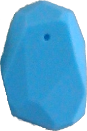
\includegraphics[scale=0.1]{Bilder/Beacon}};
\node[above left] (P1) at (Beacon1) {$P_1$};
\node[anchor=mid,inner sep=0] (Beacon2) at (6,0){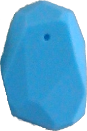
\includegraphics[scale=0.1]{Bilder/Beacon}};
\node[above right] (P2) at (Beacon2) {$P_2$};
\node[anchor=mid,inner sep=0] (Beacon3) at (3,5){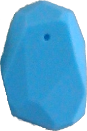
\includegraphics[scale=0.1]{Bilder/Beacon}};
\node[above right] (P3) at (Beacon3) {$P_3$};
\node[anchor=mid,inner sep=0] (MotoG) at (3,2.1){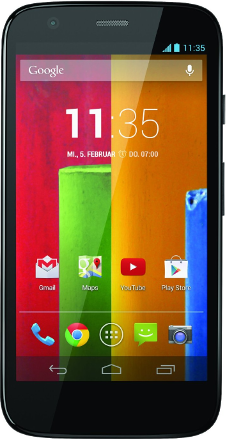
\includegraphics[scale=0.04]{Bilder/MotoG}};
\node[above right, inner sep=6] (P4) at (MotoG) {$P_{Inter}$};
\draw [thick, ->] (Beacon1) -- node[above] {$r_1$} ++(MotoG);
\draw [thick, ->] (Beacon2) -- node[above] {$r_2$} ++(MotoG);
\draw [thick, ->] (Beacon3) -- node[right] {$r_3$} ++(MotoG);
\end{tikzpicture}
\caption{Beispiel einer Trilateration zur Positionsbestimmung}
\label{fig:Trilat}
\end{wrapfigure}
Im Gegensatz zur relativen Lokalisierung mittels Lagebeschreibung, existiert noch die Methode der Mikro-Lokalisierung. Diese berechnet eine genaue Distanz zu einem Beacon und letztlich kann mithilfe von zusätzlichen Signalen mehrerer Beacons eine genaue Lokalisierung mit Koordinaten im Raum  durchgeführt werden. Für die Bestimmung einer Position aus den empfangenen Beacon-Signalen existieren mehrere Verfahren. Ein gängige Methode ist die Tri,- bzw. Multilateration die aus der Entfernung eines Punktes zwischen drei oder mehreren Orientierungspunkten dessen Position in einem Koordinatensystem bestimmt. In diesem Fall wären es die Positionen der Beacons, die Orientierungspunkte und die Entfernungen ließen sich aus den Signalen der Beacons berechnen. Mit einem Modell der Signalausbreitung wird dabei die Signalstärke, die durch den Weg vom Beacon zum Empfangsgerät geschwächt wurde, direkt in eine Distanz umgerechnet. Im übernächsten Kapitel wird ein solches Modell dafür beschrieben. An dieser Stelle soll noch einmal auf die Vorgehensweise zur Lokalisierung mittels Trilateration eingegangen werden. Dafür dient Abbildung \ref{fig:Trilat} zur Veranschaulichung der Lösung. Im ersten Schritt werden dazu die Positionen der Beacons zur Vereinfachung in ein neues Koordinatensystem transformiert. Dabei wird ein Beacon in den Koordinatenursprung verlegt und ein zweiter durch Rotation um die Z-Achse auf die X-Achse gesetzt.\\ \\
Translation:
\begin{align*}
T &= -P_1\\
P_1' &= P_1 + T = \binom{0}{0}\\
P_2' &= P_2 + T\\
P_3' &= P_3 + T
\end{align*} 
Rotation:
\begin{align*}
\alpha &= -\arcsin \left ( \frac{y_2}{\sqrt{x_2^2+y_2^2}} \right )\\
R_z\left ( \alpha \right ) &= \begin{bmatrix}
\cos\left ( \alpha \right ) & -\sin\left ( \alpha \right )\\ 
\sin\left ( \alpha \right ) & \cos\left ( \alpha \right )
\end{bmatrix}\\
P_1'' &= \binom{0}{0}\\
P_2'' &= R_z\left ( \alpha \right ) \cdot P_2'\\
P_3'' &= R_z\left ( \alpha \right ) \cdot P_3'
\end{align*}
Anhand zweier Formeln lassen sich dann die Koordinaten des Empfangsgeräts aus den einzelnen Distanzen berechnen und schließlich ins ursprüngliche Koordinatensystem zurück transformieren \cite{Trilat}. Die Distanzen sind dabei gegeben als $r_1$, $r_2$ und $r_3$ und die Koordinaten entprechen der Nummerierung der Punkte nach der Transformation.
\begin{align*}
x_{Inter} &= \frac{r_1^2-r_2^2+x_2^2}{2x_2^2}\\
y_{Inter} &= \frac{r_1^2-r_3^2+x_3^2+y_3^2}{2y_3^2}-\frac{x_3}{y_3}\cdot x_{Inter}
\end{align*}
Rücktransformation:
\begin{align*}
P_{Inter} = R_z\left ( -\alpha \right ) \cdot \binom{x_{Inter}}{y_{Inter}} - T
\end{align*}
Ein großer Nachteil von dieser Methode ist die große Fehleranfälligkeit der Signalübertragung. In der Anwendung in Gebäuden werden die Signale oftmals von Wänden reflektiert oder gedämpft, während die hohe Dichte von Signalquellen weitere Interferenzen verursacht. Um diese Nachteile auszugleichen wird statt der Trilateration eine Multilateration angewendet. Durch die Nutzung mehrerer Beacons können Messrauschen und Störungen zum Teil ausgeglichen und die Genauigkeit der Lokalisierung somit erhöht werden. Jedoch kann in dieser Arbeit nicht auf dieses Verfahren eingegangen werden, da lediglich drei Beacons zur Verfügung standen. 

\section{Anwendungsbereiche der Indoor-Lokalisierung}
Der Bedarf an einer innerräumlichen Ortung ist normalerweise dort vorhanden, wo es für den Besucher schwer ist sich zu orientieren. Dies können große Gebäudekomplexe sein oder verwinkelte und unüberschaubare Gänge. Infolge der Digitalisierung der Gesellschaft, oft bezeichnet als "`Digitale Revolution"' oder auch unter anderem Kontext als "`Zweite Moderne"' \cite{DigRev}, entstehen durch den großen Grad der Verbreitung von mobilen "`smarten"' Geräten riesige Netzwerke mit einer schier unendlichen Datenflut. Dies eröffnet folglich eine Möglichkeit zur Kommunikation zwischen Mensch und Gebäude, in der die Beacons als "`Sinne"' des Gebäudes verstanden werden können.  
\subsection{Mögliche Einsatzszenarien}
\begin{wrapfigure}{r}{9cm} 
\centering
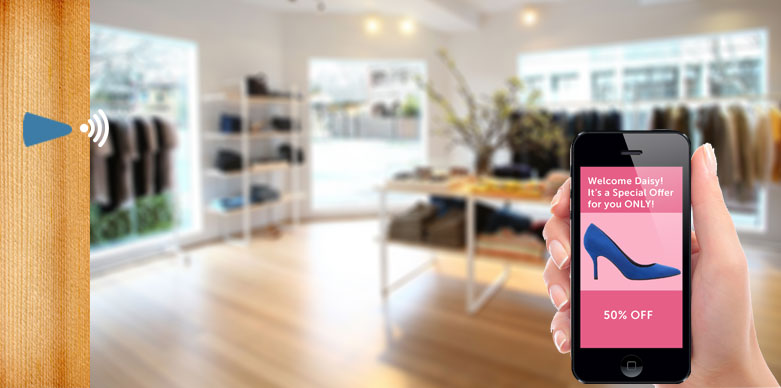
\includegraphics[scale=0.3]{Bilder/iBeaconShoe}
\caption{Beacon Nutzung in Geschäften \cite{Shoe}}
\label{fig:Shoe}
\end{wrapfigure}
Viele Unternehmen nutzen hier die Möglichkeiten einer vernetzten Welt, um besser das Verhalten der Kundschaft zu verstehen. Um wieder auf das Beispiel von der Warenhauskette zurück zu kommen, wäre es für das Unternehmen von Vorteil, zu wissen, wie viele Kunden am Tag eine Filiale besuchen, wie ihr Bewegungsprofil aussieht und was sie am Ende kaufen. Nützlich wären die Informationen für die Preisgestaltung, den Aufbau der Abteilungen im Warenhaus und dies könnte auch zu einer besseren "`Just-In-Time"' Lieferkette führen und somit Lagerkapazitäten einsparen. Natürlich wäre dies auch mit herkömmlichen Methoden möglich, indem Umfragen stattfinden und die Mitarbeiter eines Gechäftes die Kunden genau beobachten würden. Dies wäre aufgrund hoher Personalkosten nicht nur unrentabel, sondern würde den Kunden außerdem ein Gefühl der Überwachung vermitteln. Mit der Beacon-Technologie wäre dies kostengünstig und voll automatisiert möglich. Damit potentielle Kunden auch die dafür nötige Software für ihr mobiles Endgerät installieren und an der Auswertung ihrer Daten zustimmen, können die Kunden mit einer entsprechenden Applikation an exklusiven Gewinnspielen, Rabattaktionen oder Punktesystemen teilnehmen, so wie es heute schon durch einige Unternehmen angeboten wird (z.B. DeutschlandCard\footnote{\url{www.deutschlandcard.de}}, Payback\footnote{\url{www.payback.de}}, etc.). Die gesellschaftliche Akzeptanz wäre sicherlich gegeben, da es schon mit den modernen Stauwarnsystemen einen Vergleichfalls im Outdoor-Bereich gibt. Da die Position eines Fahrzeuges entweder durch das eingebaute Navigationssystem bekannt oder durch die Mobilfunkgeräte der Fahrzeuginsassen ermittelt werden kann, werden schon heute diese Systeme zur Erschaffung von Bewegungsprofilen und damit zur Stauvorhersage genutzt \cite{Stau}. Für ein solches Szenario im Indoor-Bereich würde hauptsächlich die kontextbezogene Lokalisierung in Betracht gezogen werden, da hier die meisten Geschäfte überschaubar sind und schon gute Strukturen zur Orientierung der Kundschaft genutzt werden. Extreme Ausnahmen wie die "`Golden Resources Mall"' in Peking mit 557,419 $\text{m}^2$ Ladenfläche, wo eine genauere Lokalisierung zur Navigation sicherlich sinnvoll wäre, bilden hier eher die Ausnahme. \par\bigskip
\begin{wrapfigure}{l}{8.5cm} 
\centering
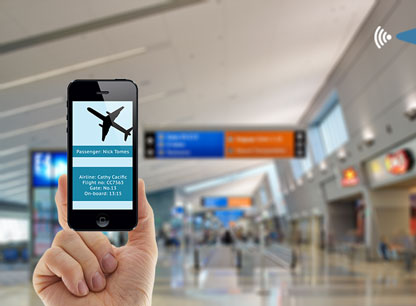
\includegraphics[scale=0.5]{Bilder/iBeaconAirport}
\caption{Beacon Nutzung im Flughäfen \cite{Airpo}}
\label{Airpo}
\end{wrapfigure}
Im Gegensatz dazu stellt die Mikro-Lokalisierung ein weiteres mögliches Szenario dar. Sie soll dazu dienen Menschen oder Objekte genau zu lokalisieren, um unter Verwendung von speziellen Applikationen eine bessere Orientierung zu gewährleisten. Daran interessiert sind meist Branchen, die ihre Kundschaft gerne schnell und ohne Umwege zu dem führen möchten, weswegen sie in die Einrichtung des Unternehmens gekommen sind. Als Beispiele können hier Messehallen- und Flughafenbetreiber genannt werden. In diesen Branchen sind die Gebäude meistens sehr unübersichtlich und die Kundschaft ist häufig ortsfremd. Der Vorteil den die Unternehmen aus dem System ziehen können, ist eine bessere Verteilung der Kunden durch eine intelligente Pfadplanung. So können die Platzkapazitäten der Einrichtungen besser genutzt und die Gäste somit schneller abgefertigt werden. Wenn zudem ein Unternehmen in seinen Gebäuden eine ähnliches System wie ein Navigationssystem für die Straße bieten kann, bedeutet dies auch einen Wettbewerbsvorteil und fördert die Kundenzufriedenheit. \\ \\
Grundsätzlich sind dies hier nur Annahmen für mögliche Szenarien. Da es noch keine praktikablen Anwendungen der Indoor-Lokalisierung gibt, können keine genauen Vorhersagen diesbezüglich getroffen werden. Viele Unternehmen schrecken noch davor ab, weil kein einheitlicher Standard existiert und nur wenige Menschen mit der Technik vertraut sind. \par\bigskip 
\subsection{Planungskonzepte für Beacon-Konfigurationen}
Bisherige Ansätze um ein Lokalisierungssystem in einem Raum zu realisieren beruhen auf fachmännischen Einschätzungen des Beacon-Installateurs. Das bedeutet, dass sich das Konzept lediglich auf Erfahrungswerte beruft. Die Beacons werden dabei an strategische Punkte gesetzt und manuell an jeder Postion neu konfiguriert. Wie schon oben beschrieben, werden die Befestigungen der Beacons im Raum vermessen oder grob geschätzt und so zur Positionsbestimmung in eine Lokalisierungs-Applikation ebenfalls wieder manuell eingepflegt. Von der Firma Estimote gibt es seit Neuestem eine neue Applikation namens "`Estimote Indoor Location "', die den Entwicklern einer Lokalisierungs-Applikation unterstützen soll. Der Entwickler installiert dazu an jeder der vier Wände eines Raumes ein Beacon der Firma und ausgehend vom Eingang startet der Entwickler die App und läuft anschließend den ganzen Raum ab. Dabei werden die Signale der Beacons an den Wänden aufgezeichnet und mithilfe der inertialen Sensoren des Smartphones zusätzlich die Bewegungsinformationen gespeichert. Daraus errechnet die App eine Karte vom Raum und liefert auch gleich eien Positionsbestimmung mithilfe der genannten Sensordaten in Echtzeit. Diese Karte kann auch in Eigenentwicklungen für das Smartphone verwendet werden, jedoch ist dafür eine Migration der Daten notwendig. Da für diese Arbeit nur drei Beacons zur Verfügung standen und diese App erst in der späten Phase der Arbeit veröffentlicht wurde, wird hier nicht mehr auf dieses Konzept eingegangen werden. Jedoch lassen die noch engen Begrenzungen der Anwendung (konstante Anzahl von vier Beacons, Einstellung der Parameter wieder manuell nach Erfahrungswert) keinen Handlungsspielraum für die Optimierung der Beacon-Konfigurationen zu. Zudem muss immer ein Entwickler die Räume ablaufen und später die Daten vom Smartphone in die eigene Entwicklung migrieren. Für kleine Räume ist diese Strategie sicherlich hilfreich, jedoch wird sie bei Großprojekten, wie z.B. die Schaffung eines Ortungssystems in einem Flughafen schlicht unbrauchbar.
\begin{figure}[H]
\centering
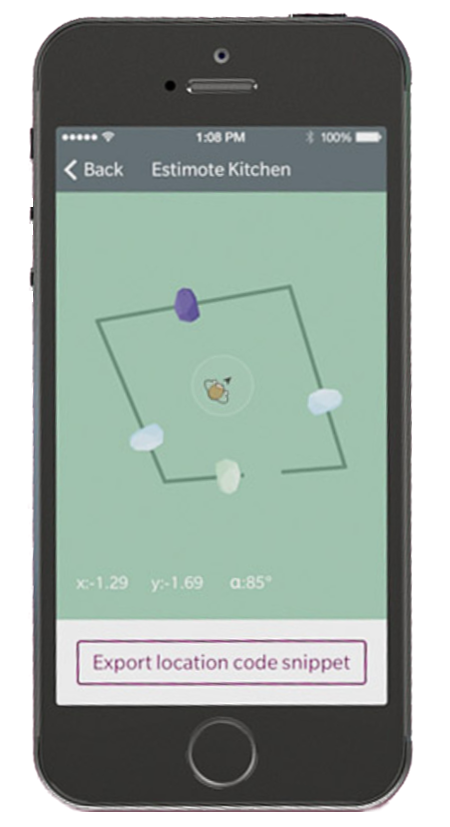
\includegraphics[scale=0.3]{Bilder/TrackEstimote}
\caption{Demo der Estimote Indoor Localization App \cite{TrEs}}
\end{figure}